% To be compiled by XeLaTeX, preferably under TeX Live.
% LaTeX source for ``Yanqi Lake Lectures on Algebra'' Part III.
% Copyright 2019  李文威 (Wen-Wei Li).
% Permission is granted to copy, distribute and/or modify this
% document under the terms of the Creative Commons
% Attribution-NonCommercial 4.0 International (CC BY-NC 4.0)
% https://creativecommons.org/licenses/by-nc/4.0/

% To be included
\chapter*{Introduction}
\addcontentsline{toc}{chapter}{Introduction}
\markboth{Introduction}{}

In the beginning, these lecture notes were prepared for the graduate course \emph{Algebra III} (ID: 011M4002Y) in Spring 2016, University of the Chinese Academy of Sciences. For some reasons, it took place in the Yuquanlu campus instead of the Yanqi Lake campus as it should be.

The course is a sequel to Algebra I (fields, modules and representations) and II (homological algebra). The topic of this Part III is commutative algebra, or more precisely \emph{commutative ring theory}. Each ``Lecture'' in these notes took roughly one week, say approximately four hours of lecture, but the materials were only partially covered. My initial intention was to give a traditional course on commutative algebra as proposed by the syllabus prescribed by UCAS. For various reasons, my plan failed. For example, there are too few discussions on depth, regular sequences and Cohen--Macaulay modules, too few applications of completions, and the computational aspects haven't been touched. Moreover, the homological aspect of commutative algebra is almost non-existent in these notes, namely the Auslander--Buchsbaum Formula, the properties of regular local rings, etc. Last but not least, the exercises herein are scarcely sufficient.

These notes were also used for the Enhanced Program for Graduate Study held at the Beijing International Center of Mathematical Research, Peking University, during Spring 2019 (course ID: 00102057).

As the title suggests, some backgrounds from the Part I are presumed, namely the basic notions of rings, modules and their chain conditions, as well as familiarity with tensor products and some Galois theory. We occasionally presume some basic knowledge of homological algebra, such as the functors $\Tor_i$ and $\Ext^i$.

Sometimes I made free use of the language of derived categories. This was indeed covered in the preceding course \emph{Algebra II}, and it should be common sense for the future generations.

As the reader might have observed, these notes were prepared in a rush; certain paragraphs have not been proofread yet and many proofs are silly. I am very grateful to the students for various corrections and improvements, and I will try to polish these notes in the future.

\section*{Conventions}
Throughout these lectures, we consider only associative rings with unit $1$, and the rings and algebras are assumed to be commutative and nonzero unless otherwise specified. The ideal generated by elements $x_1, x_2, \ldots$ in a ring $R$ is denoted by $(x_1, x_2, \ldots)$ or sometimes $\langle x_1, x_2, \ldots \rangle$; the $R$-algebra of polynomials in variables $X, Y, \ldots$ with coefficients in $R$ is denoted by $R[X, Y, \ldots]$. We write $R^\times$ for the group of invertible elements in a ring $R$. A ring without zero-divisors except $0$ is called an integral domain, or simply a domain. The localization of a ring $R$ with respect to a multiplicative subset $S$ will be written as $R[S^{-1}]$.

For any sets $E, F$, let $E \smallsetminus F := \left\{ x \in E: x \notin F \right\}$. The cardinality of $E$ is denoted by $|E|$.

The usual logical connectives such as $\exists$, $\forall$, $\wedge$, $\vee$ and so forth will occasionally be used. Writing $A := B$ means that the expression $A$ is defined to be $B$.

We will use the standard notations $\Z, \Q, \R, \CC$ to denote the set of integers, of rational numbers, etc. Sans serif fonts are reserved for categories, such as $\cate{Ab}$ (abelian groups) and $\cate{Ring}$. 

When denoting morphisms in a category by arrows, monomorphisms (resp.\ epimorphisms, isomorphisms) will be indicated $\hookrightarrow$ (resp.\ $\twoheadrightarrow, \rightiso$).

\section*{Possible references}
The reader is expected to have basic familiarity with groups, rings and modules, as covered in my lecture notes on Algebra I. We will make use of some really elementary homological algebra as our course proceeds --- so keep calm.

Our main references will be \cite{Mat80} and \cite{Eis95}. The Bourbaki volumes \cite{Bour83, Bour98} serve as our ultimate source. The readers are also encouraged to consult the relevant materials in \href{https://stacks.math.columbia.edu/}{Stacks Project}.

\vfill
\begin{figure}[h]
	\centering 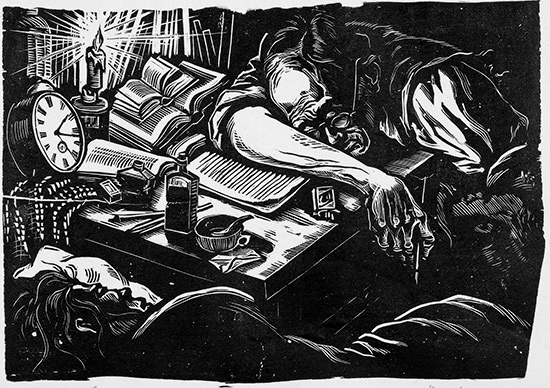
\includegraphics[height=180pt]{JiaoShouShengYa.jpg} \\ \vspace{1em}
	\begin{minipage}{0.7\textwidth}\begin{center}
		\small \fontspec{Noto Serif CJK SC} 《教授生涯》, 李桦, 木刻版画, 1948 年.
	\end{center}\end{minipage}
\end{figure}
\vfill